
%======================问题介绍====================================
\section{Introduction}

Although a hitter might expect a model of the bat–baseball collision to
yield insight into how the bat breaks, how the bat imparts spin on the ball,
how best to swing the bat, and so on, we model only the sweet spot.

There are at least two notions of where the sweet spot should be—an
impact location on the bat that either
\begin{itemize}
\item minimizes the discomfort to the hands, or
\item maximizes the outgoing velocity of the ball.
\end{itemize}
We focus exclusively on the second definition.

\begin{itemize}
  \item the initial velocity and rotation of the ball,
\item the initial velocity and rotation of the bat,
\item the relative position and orientation of the bat and ball, and
\item the force over time that the hitter抯 hands applies on the handle.
\end{itemize}
We assume that the ball is not rotating and that its velocity at impact is
perpendicular to the length of the bat. We assume that everything occurs
in a single plane, and we will argue that the hands?interaction is negligible.
In the frame of reference of the center of mass of the bat, the initial conditions
are completely specified by
\begin{itemize}
  \item the angular velocity of the bat,
\item the velocity of the ball, and
\item the position of impact along the bat.
\end{itemize}
The location of the sweet spot depends not on just the bat alone but also
on the pitch and on the swing.
The simplest model for the physics involved has the sweet spot at the
\emph{center of percussion} [Brody 1986], the impact location that minimizes discomfort
to the hand. The model assumes the ball to be a rigid body for which
there are conjugate points: An impact at one will exactly balance the angular
recoil and linear recoil at the other. By gripping at one and impacting at the
other (the center of percussion), the hands experience minimal shock and
the ball exits with high velocity. The center of percussion depends heavily
on the moment of inertia and the location of the hands. We cannot accept
this model because it both erroneously equates the two definitions of sweet
spot and furthermore assumes incorrectly that the bat is a rigid body.
Another model predicts the sweet spot to be between nodes of the two
lowest natural frequencies of the bat [Nathan 2000]. Given a free bat allowed
to oscillate, its oscillations can be decomposed into fundamental
modes of various frequencies. Different geometries and materials have different
natural frequencies of oscillation. The resulting wave shapes suggest
how to excite those modes (e.g., plucking a string at the node of a vibrational
mode will not excite that mode).




    \begin{Theorem} \label{thm:latex}
    \LaTeX
    \end{Theorem}
    \begin{Lemma} \label{thm:tex}
    \TeX .
    \end{Lemma}
    \begin{proof}
    The proof of theorem.
    \end{proof}






\subsection{Other Assumptions}
%\renewcommand{\labelitemi}{\ding{43}}
Although Mr. Gore has expressed concerns to some associates about
the damage a brokered convention could cause, several associates
said he was hopeful that one candidate would soon break through,
sparing the party such an outcome. He told a close friend recently
that his decision not to endorse “feels like the right thing”
and that he remained optimistic the race “is going to tip at some
point,” the friend said.
\begin{itemize}
\item
\item
\item
\item
\end{itemize}

 Under the above and basic assumptions, we can set out
to construct our model (show our approach in detail).
%=============================问题分析==========================================
\section{Analysis of the Problem }
%==================================模型建立==============================================
\begin{figure}
\small
\centering
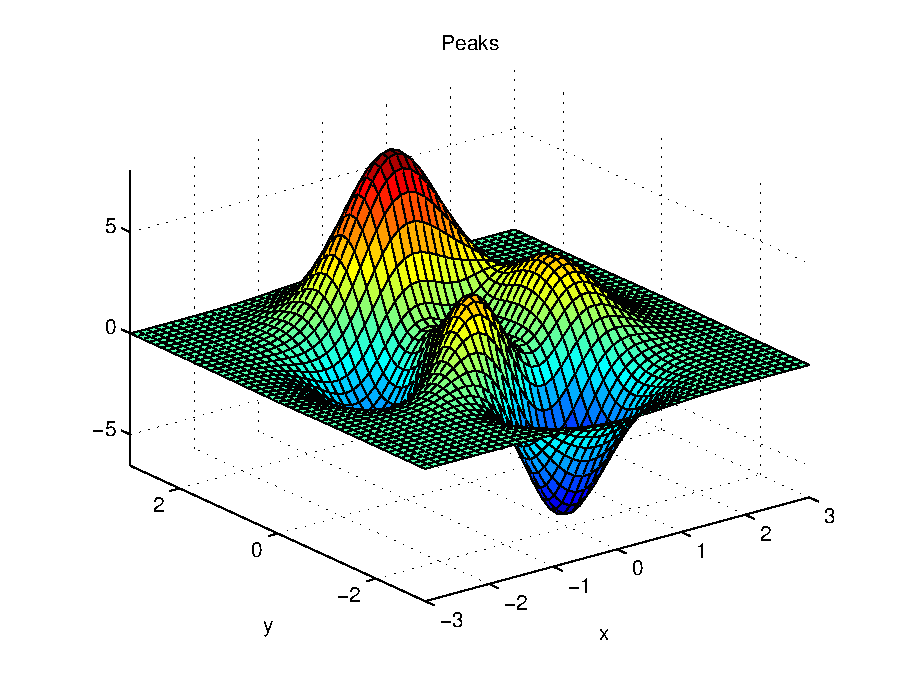
\includegraphics[width=12cm]{./picture/aaa.eps}
\caption{aa} \label{fig:aa}
\end{figure}

Although Mr. Gore has expressed concerns to some associates about
the damage a brokered convention could cause, several associates
said he was hopeful that one candidate would soon break through,
sparing the party such an outcome. He told a close friend recently
that his decision not to endorse “feels like the right thing”
and that he remained optimistic the race “is going to tip at some
point,” the friend said.\eqref{aa}
\begin{equation}
  a^2 \label{aa}
\end{equation}


\[
\left( {\begin{array}{*{20}c}
   {a_{11} } & {a_{12} } & {a_{13} }  \\
   {a_{21} } & {a_{22} } & {a_{23} }  \\
   {a_{31} } & {a_{32} } & {a_{33} }  \\
\end{array}} \right) = \frac{{Opposite}}{{Hypotenuse}}\cos ^{ - 1} \theta \arcsin \theta
\]
Although Mr. Gore has expressed concerns to some associates about
the damage a brokered convention could cause, several associates
said he was hopeful that one candidate would soon break through,
sparing the party such an outcome. He told a close friend recently
that his decision not to endorse “feels like the right thing”
and that he remained optimistic the race “is going to tip at some
point,” the friend said.

\[
p_{j}=\begin{cases} 0,&\text{if $j$ is odd}\\
r!\,(-1)^{j/2},&\text{if $j$ is even}
\end{cases}
\]
Although Mr. Gore has expressed concerns to some associates about
the damage a brokered convention could cause, several associates
said he was hopeful that one candidate would soon break through,
sparing the party such an outcome. He told a close friend recently
that his decision not to endorse “feels like the right thing”
and that he remained optimistic the race “is going to tip at some
point,” the friend said.
\[
\arcsin \theta  =
\mathop{{\int\!\!\!\!\!\int\!\!\!\!\!\int}\mkern-31.2mu
\bigodot}\limits_\varphi
 {\mathop {\lim }\limits_{x \to \infty } \frac{{n!}}{{r!\left( {n - r}
 \right)!}}} \eqno (1)
\]




\section{Calculating and Simplifying the Model  } ``A is equivalent
to B'' Although Mr. Gore has expressed concerns to some associates
about the damage a brokered convention could cause, several
associates said he was hopeful that one candidate would soon break
through, sparing the party such an outcome. He told a close friend
recently that his decision not to endorse “feels like the right
thing” and that he remained optimistic the race “is going to tip
at some point,” the friend said.



%===============================模型结果============================================
\section{The Model Results}
Although Mr. Gore has expressed concerns to some associates about
the damage a brokered convention could cause, several associates
said he was hopeful that one candidate would soon break through,
sparing the party such an outcome. He told a close friend recently
that his decision not to endorse “feels like the right thing”
and that he remained optimistic the race “is going to tip at some
point,” the friend said.


%========================模型的实效分析(适应性说明)=============================

\section{Validating the Model}%确认模型,使之合理。
Although Mr. Gore has expressed concerns to some associates about
the damage a brokered convention could cause, several associates
said he was hopeful that one candidate would soon break through,
sparing the party such an outcome. He told a close friend recently
that his decision not to endorse “feels like the right thing”
and that he remained optimistic the race “is going to tip at some
point,” the friend said. Although Mr. Gore has expressed concerns
to some associates about the damage a brokered convention could
cause, several associates said he was hopeful that one candidate
would soon break through, sparing the party such an outcome. He
told a close friend recently that his decision not to endorse
“feels like the right thing” and that he remained optimistic the
race “is going to tip at some point,” the friend said.


Although Mr. Gore has expressed concerns to some associates about
the damage a brokered convention could cause, several associates
said he was hopeful that one candidate would soon break through,
sparing the party such an outcome. He told a close friend recently
that his decision not to endorse “feels like the right thing”
and that he remained optimistic the race “is going to tip at some
point,” the friend said.

\section{Conclusions}
Although Mr. Gore has expressed concerns to some associates about
the damage a brokered convention could cause, several associates
said he was hopeful that one candidate would soon break through,
sparing the party such an outcome. He told a close friend recently
that his decision not to endorse “feels like the right thing”
and that he remained optimistic the race “is going to tip at some
point,” the friend said.
\section{A Summary    }
Although Mr. Gore has expressed concerns to some associates about
the damage a brokered convention could cause, several associates
said he was hopeful that one candidate would soon break through,
sparing the party such an outcome. He told a close friend recently
that his decision not to endorse “feels like the right thing”
and that he remained optimistic the race “is going to tip at some
point,” the friend said.
%================================总体评价==============================
\section{Evaluate of the Mode}

%======================================================================
\section{Strengths and weaknesses}
Like any model,the one present above has its strengths and
weaknesses. Some of the major points are presented below.

%============================模型=优点====================================
\subsection{Strengths}
\begin{itemize}
\item \textbf{Applies widely}\\
This  system can be used for many types of airplanes, and it also
solves the interference during  the procedure of the boarding
airplane,as described above we can get to the  optimization
boarding time.We also know that all the service is automate.
\item \textbf{Improve the quality of the airport service}\\
Balancing the cost of the cost and the benefit, it will bring in
more convenient  for airport and passengers.It also saves many
human resources for the airline. \item \textbf{}
\end{itemize}




\begin{thebibliography}{99}
%\addcontentsline{toc}{section}{References}
\bibitem{1} D. E. KNUTH   The \TeX{}book  the American
Mathematical Society and Addison–Wesley
Publishing Company , 1984-1986.
\bibitem{2}Lamport, Leslie,  \LaTeX{}: `` A Document Preparation System '',
Addison-Wesley Publishing Company, 1986.
\bibitem{3}http://www.latexstudio.net/
\bibitem{4}http://www.chinatex.org/
\end{thebibliography}

%====================附录导入程序代码==========================================
\begin{appendices}
    %\renewcommand{\thesection}{\Alph{chapter}.}

\section{First appendix}

some text...


Here are simulation programmes we used in our model as follow.\\


\textbf{\textcolor[rgb]{0.98,0.00,0.00}{Input matlab source:}}
\lstinputlisting[language=Matlab]{./code/matlab1.m}


      \section{Second appendix}

    some more text\textcolor[rgb]{0.98,0.00,0.00}{\textbf{Input C++ source:}}
\lstinputlisting[language=C++]{./code/sudoku.cpp}

    \end{appendices}
